% 基于大数据架构的电影搜索与推荐系统 —— 课程汇报 slides v2（editorial / anti-AI-flavor）
% 编译: xelatex -enable-installer -interaction=nonstopmode slides.tex （跑两遍）
\documentclass[aspectratio=169,11pt,fontset=none]{ctexbeamer}
\usepackage{booktabs}
\usepackage{caption}
\usepackage{colortbl}
\usepackage{tikz}
\usetikzlibrary{arrows.meta,positioning}
\graphicspath{{../experiments/screenshots/}}

% ---------- 字体 ----------
\setCJKmainfont{Microsoft YaHei}
\setCJKsansfont{Microsoft YaHei}
\setmainfont{Segoe UI}
\setsansfont{Segoe UI}
\setmonofont{Consolas}[Scale=0.92]

% ---------- 色板：纸白 / 墨黑 / 国际橙 ----------
\definecolor{ink}{HTML}{181614}
\definecolor{paper}{HTML}{FAF8F3}
\definecolor{accent}{HTML}{E8500F}
\definecolor{mute}{HTML}{8B857A}
\definecolor{line}{HTML}{DAD4C8}
\definecolor{cellbg}{HTML}{FFFFFF}
\definecolor{darkfg}{HTML}{F5F1E8}

\usetheme{default}
\setbeamertemplate{navigation symbols}{}
\setbeamercolor{background canvas}{bg=paper}
\setbeamercolor{normal text}{fg=ink}
\setbeamercolor{structure}{fg=ink}
\setbeamercolor{alerted text}{fg=accent}
\setbeamercolor{itemize item}{fg=accent}
\setbeamercolor{itemize subitem}{fg=mute}
\setbeamertemplate{itemize item}{\textcolor{accent}{\rule[0.1em]{0.55em}{0.09em}}}
\setbeamertemplate{itemize subitem}{\textcolor{mute}{\rule[0.1em]{0.4em}{0.09em}}}
\setbeamercolor{enumerate item}{fg=accent}

\setbeamertemplate{frametitle}{%
  \vspace{5pt}%
  {\LARGE\bfseries\insertframetitle}\par
  \vspace{3pt}{\color{line}\rule{\textwidth}{0.7pt}}\par
  \vspace{2pt}}

\setbeamertemplate{footline}{%
  \leavevmode\hbox{%
    {\color{mute}\tiny\texttt{\hspace{8pt}movie-search-rec / 课程汇报}}\hfill
    {\color{mute}\tiny\texttt{\insertframenumber\,/\,\inserttotalframenumber\hspace{8pt}}}}\vspace{5pt}}

\newcommand{\kicker}[1]{{\color{mute}\footnotesize\texttt{\MakeUppercase{#1}}}\par\vspace{1pt}}
\newcommand{\stat}[3][26]{{\fontsize{#1}{\numexpr#1+2\relax}\selectfont\bfseries\textcolor{accent}{\texttt{#2}}}\\[1pt]{\color{mute}\small #3}\par}
\newcommand{\mono}[1]{\texttt{#1}}
\newcommand{\cellbox}[2]{\fcolorbox{line}{cellbg}{\parbox[t][#1][t]{\dimexpr\linewidth-2\fboxsep-0.4pt\relax}{#2}}}
\newcommand{\darkpage}{%
  \setbeamercolor{background canvas}{bg=ink}%
  \setbeamercolor{normal text}{fg=darkfg}%
  \setbeamercolor{frametitle}{fg=darkfg}}
\newcommand{\lightpage}{%
  \setbeamercolor{background canvas}{bg=paper}%
  \setbeamercolor{normal text}{fg=ink}%
  \setbeamercolor{frametitle}{fg=ink}}
\newcommand{\divider}[2]{%
{\darkpage
\begin{frame}[plain]
  \color{darkfg}
  \vspace{8mm}
  {\fontsize{64}{64}\selectfont\bfseries\textcolor{accent}{\texttt{#1}}}\\[6pt]
  {\fontsize{34}{38}\selectfont\bfseries #2}
  \vfill
  {\color{mute}\small\texttt{section #1 / 06}}
  \vspace{6mm}
\end{frame}}}

\title{基于大数据架构的电影搜索与推荐系统}
\begin{document}

% ================= 封面（暗页） =================
{\darkpage
\begin{frame}[plain]
  \vspace{6mm}
  {\color{accent}\rule{28pt}{5pt}}\par\vspace{12pt}
  {\color{darkfg}\fontsize{30}{36}\selectfont\bfseries 基于大数据架构的\\[4pt] 电影搜索与推荐系统\textcolor{accent}{.}}\par\vspace{12pt}
  {\color{mute}\large 2500 万条评分的召回、排序与生成式推荐，\\[2pt] 从三节点集群到一个能打开的网页}
  \vfill
  {\color{darkfg}\footnotesize\texttt{MovieLens 25M ~~·~~ Hadoop 3.3.6 / Hive 4.0.1 / Spark 3.5.9 ~~·~~ CPU only}}\\[4pt]
  {\color{mute}\footnotesize （姓名 · 学号）\hfill 2026 年 11 月}
  \vspace{5mm}
\end{frame}}

% ================= 目录 =================
\begin{frame}[plain]
  \frametitle{这次汇报讲什么}
  \vspace{4pt}
  \begin{columns}[T]
    \column{0.08\textwidth}\color{accent}\rule{2pt}{52mm}
    \column{0.88\textwidth}
    {\large
    \texttt{\textcolor{accent}{01}}\quad 项目介绍：要做什么，约束是什么\\[11pt]
    \texttt{\textcolor{accent}{02}}\quad 设计实现：集群、数仓、六类模型、一个服务\\[11pt]
    \texttt{\textcolor{accent}{03}}\quad 实验结果：同一考卷的总表，和拆零件的消融\\[11pt]
    \texttt{\textcolor{accent}{04}}\quad 项目总结：亮点、教训、没做完的\\[11pt]
    \texttt{\textcolor{accent}{05}}\quad 成员分工\\[11pt]
    \texttt{\textcolor{accent}{06}}\quad 资源链接与复现方式}
  \end{columns}
\end{frame}

% =====================================================
\divider{01}{项目介绍}

\begin{frame}{要做什么}
  \kicker{one-liner}
  在自建的三节点 Hadoop 集群上，给 MovieLens 的 2500 万条评分搭一套完整的搜推系统：数据进 Hive 数仓，六类模型在集群上训练，评测用同一份考卷，最后包成一个浏览器里能点的网页服务。

  \vspace{10pt}
  \begin{columns}[T]
    \column{0.31\textwidth}\cellbox{17mm}{\centering\vspace{2pt}\stat[20]{25{,}000{,}095}{条评分}}
    \column{0.31\textwidth}\cellbox{17mm}{\centering\vspace{2pt}\stat{162{,}541}{个用户，全量参加考试}}
    \column{0.31\textwidth}\cellbox{17mm}{\centering\vspace{2pt}\stat{62{,}423}{部电影，全量候选集}}
  \end{columns}

  \vspace{10pt}\small
  课程知识点的落点：协同过滤在召回层（ALS、ItemCF），分类在精排层（LR/FM/DeepFM），回归是独立的热度预测模块，聚类落在语义 ID 的 RQ 量化里；自建 Linux 集群与生成式推荐属于加分项，都做了。
\end{frame}

\begin{frame}{流水线长这样}
  \centering
  \begin{tikzpicture}[node distance=4mm and 5mm,
      box/.style={draw=ink,fill=cellbg,line width=0.7pt,inner sep=5pt,
                  font=\scriptsize\bfseries,align=center,minimum height=15mm},
      arr/.style={-{Stealth[length=2.5mm]},line width=1.1pt,accent}]
    \node[box] (data) {MovieLens 25M\\2500 万评分};
    \node[box,right=of data] (etl) {Spark ETL\\Hive ODS/DWD/DWS\\leave-last-out 切分};
    \node[box,right=of etl] (train) {模型训练\\ALS / ItemCF / SASRec\\DeepFM / GBT / SID};
    \node[box,below=9mm of train] (eval) {统一评测\\全量排序 + 消融\\RRF 融合};
    \node[box,left=of eval] (serve) {在线服务\\FastAPI 多路召回\\MMR 重排};
    \node[box,left=of serve] (web) {网页\\ECharts 看板};
    \draw[arr] (data)--(etl); \draw[arr] (etl)--(train);
    \draw[arr] (train)--(eval);
    \draw[arr] (eval)--(serve); \draw[arr] (serve)--(web);
  \end{tikzpicture}

  \vspace{8pt}\small
  生成式是另一条支线：电影内容量化成语义 ID，模型直接\alert{生成}推荐序列（TIGER / OneRec 的做法）。\\
  所有模型用同一份切分、同一套指标打分；每个零件都做消融，回答"拆掉它掉多少分"。
\end{frame}

% =====================================================
\divider{02}{设计实现}

\begin{frame}{集群：一台电脑里的三个节点}
  \begin{columns}[T]
    \column{0.52\textwidth}
    \small VMware 一台虚拟机，Docker 起 3 个容器：
    \begin{itemize}
      \item \textbf{master}：NameNode、ResourceManager，Spark 从这里提交
      \item \textbf{worker1 / worker2}：DataNode、NodeManager
      \item Hive 4.0.1 的 Metastore 放在 MySQL 8 里，HBase 2.6.1 配 ZooKeeper
    \end{itemize}
    \vspace{6pt}
    一个省时间的细节：把 Spark 的依赖 jar 打成一个包传到 HDFS（\mono{spark.yarn.archive}），作业启动时不用再分发包，等待从分钟级降到秒级。
    \column{0.44\textwidth}
    \centering
    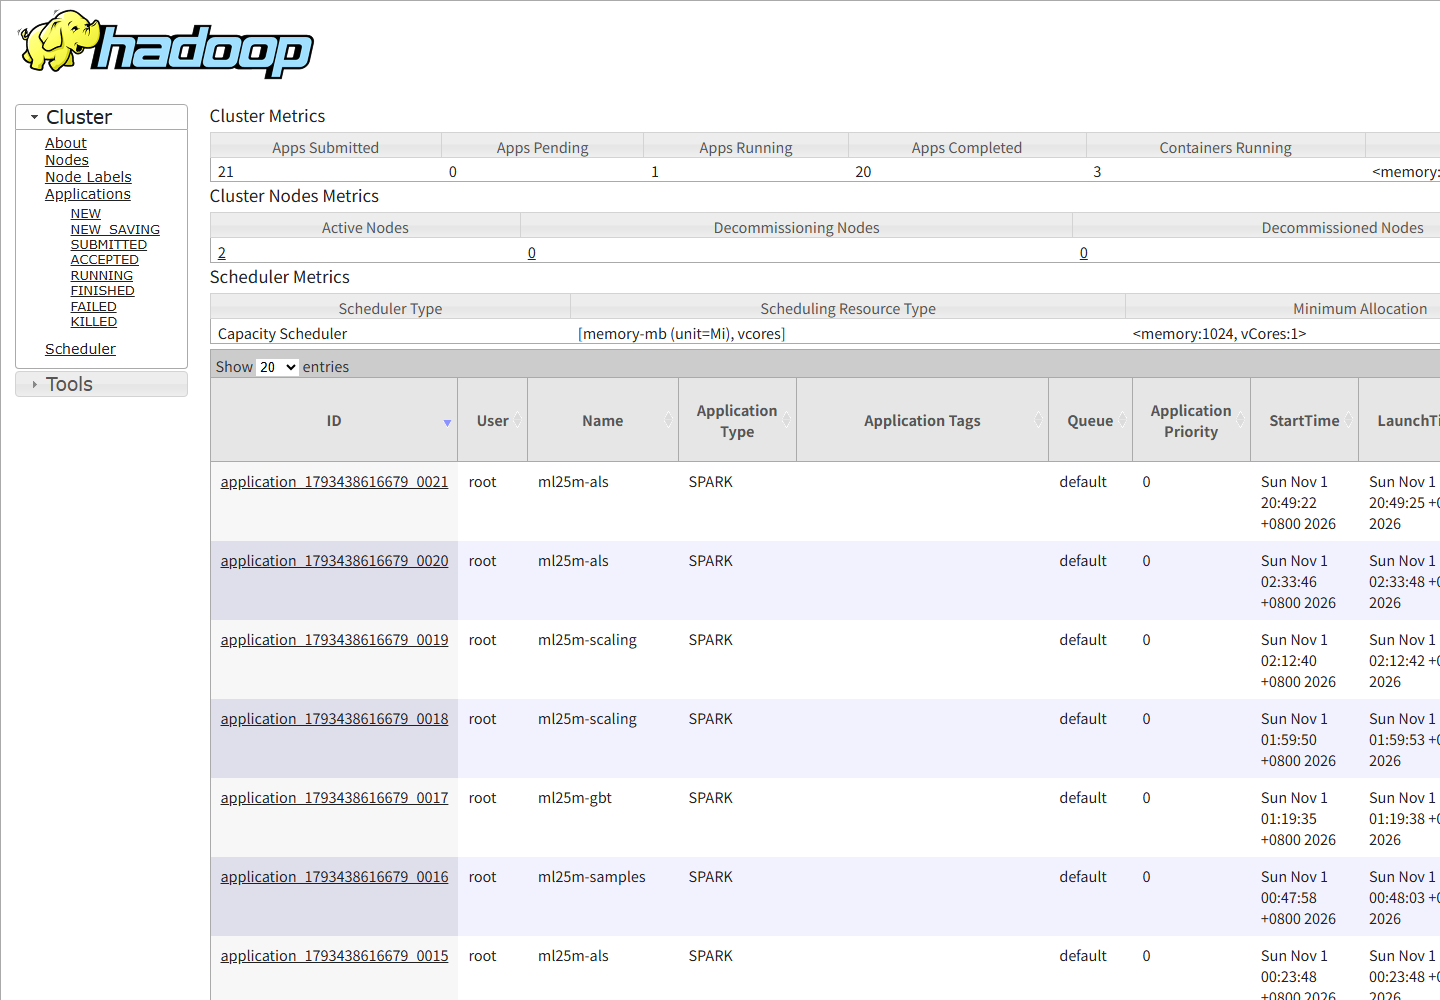
\includegraphics[width=\linewidth]{yarn_running_app.png}\\[2pt]
    {\color{mute}\footnotesize YARN 上正在跑的 ALS 训练和它前面的 20 个作业}
  \end{columns}
\end{frame}

\begin{frame}{数仓分三层，切分只做一次}
  \small
  \begin{tabular}{@{}p{0.14\textwidth}p{0.82\textwidth}@{}}
    \toprule
    \textbf{ODS} & ratings / movies / tags 原样入表，不解析，保证随时可以重放 \\
    \textbf{DWD} & Parquet 明细。正则抽标题里的年份；窗口函数做 leave-last-out：每个用户最后两条当验证和测试 \\
    \textbf{DWS} & 用户与电影统计、共现矩阵、行为序列。\alert{只看训练段的数据}，val/test 的信息不会漏进来 \\
    \bottomrule
  \end{tabular}

  \vspace{10pt}\small
  对账：25{,}000{,}095 条评分切完后，val 和 test 各 162{,}541 行，和用户数一行不差。

  \vspace{8pt}
  \cellbox{13mm}{\small\textbf{踩过一个版本坑}：Hive 4 的 Metastore Thrift 接口和 Spark 3.5 对不上，报 \mono{Invalid method name: 'get\_table'}。解法是目录解耦：以 Spark 内嵌 Derby 为准，Hive 建外部表镜像同一份数据，两边都能用 SQL 查。}
\end{frame}

\begin{frame}{召回层：四路并行，各有分工}
  \vspace{2pt}
  \begin{columns}[T]
    \column{0.49\textwidth}\cellbox{20mm}{\small\textbf{热门}\hfill{\color{mute}\scriptsize\texttt{0.06ms}}\\头部兜底、新用户冷启动，只从 Top-500 里取。}
    \column{0.49\textwidth}\cellbox{20mm}{\small\textbf{ItemCF}\hfill{\color{mute}\scriptsize\texttt{4.5ms}}\\共现 + 贡献限流，不让热门电影刷屏。}
  \end{columns}
  \vspace{5pt}
  \begin{columns}[T]
    \column{0.49\textwidth}\cellbox{24mm}{\small\textbf{ALS（隐式）}\hfill{\color{mute}\scriptsize\texttt{2.9ms}}\\$\alpha{=}40$，所有行为都算正样本。第一版用显式评分训练，R@50 只有 0.0001：它背下了"人人都爱的经典"，学不到"这个人会点开什么"。}
    \column{0.49\textwidth}\cellbox{24mm}{\small\textbf{SASRec}\hfill{\color{mute}\scriptsize\texttt{1.3ms}}\\自注意力序列模型（d64 / 2 层 / maxlen 50），拿物品嵌入向量对全量候选排序，CPU 上采样训练。}
  \end{columns}

  \vspace{8pt}\small
  四路结果用 RRF 合并：$\mathrm{score}(i)=\sum_{c}\frac{1}{60+\mathrm{rank}_c(i)}$。只看排名不看分数，天然绕开各通道分数量纲不同的问题。
\end{frame}

\begin{frame}{精排、重排，外加一个回归模块}
  \begin{columns}[T]
    \column{0.55\textwidth}
    \small
    \textbf{CTR 精排}\\[2pt]
    评分 $\ge$ 4 记为正样本，8 个特征：用户和物品的统计、年份、时间间隔、类型偏好匹配。LR、FM、DeepFM 三胞胎共用同一套特征，只换模型结构。
    \vspace{5pt}\\
    \textbf{MMR 多样性重排}\\[2pt]
    $\lambda{=}0.6$，相关性和类型多样性折中，避免首页全是同一个系列。
    \column{0.41\textwidth}
    \small
    \textbf{回归：电影热度}\\[2pt]
    用 2015--2017 年的信息预测一部电影 2018 年之后的热度。时间往后切分，不许偷看未来。GBT 对 LinearRegression，见实验部分。
  \end{columns}
  \vspace{8pt}\footnotesize\color{mute}
  精排模型在 Spark 上拼样本，PyTorch 里训练；发现过拟合后改成按验证集挑检查点，这个弯路记在总结里。
\end{frame}

\begin{frame}{生成式分支：把推荐变成"生成"}
  \begin{columns}[T]
    \column{0.52\textwidth}
    \small
    \textbf{第一步，造语义 ID}\\[2pt]
    标题、类型、高频标签过 MiniLM 句向量，PCA 压到 32 维，faiss 的 ResidualQuantizer 量化成 3 层 × 256 码字，不够表达的用第 4 层兜底。
    \vspace{6pt}

    \begin{columns}[T]
      \column{0.48\linewidth}\stat{100\%}{三层码字全部被用到，零坍缩}
      \column{0.48\linewidth}\stat{3.35\%}{ID 碰撞率（62423 部电影）}
    \end{columns}
    \column{0.44\textwidth}
    \small
    \textbf{第二步，学一个生成模型}\\[2pt]
    decoder-only Transformer（d128 / 4 层），把用户序列变成 SID 序列的语言建模任务。推理时束搜索沿着 SID 的 Trie 走，只在合法前缀上展开，已看过的电影进不了结果。
    \vspace{6pt}

    {\color{mute}\footnotesize 150ms/人（CPU 束搜索，含全量评估）。这是 TIGER / OneRec 那条工业路线在 CPU 集群上的一次完整落地。}
  \end{columns}
\end{frame}

\begin{frame}{怎么考：一份卷子，全员闭卷}
  \begin{columns}[T]
    \column{0.5\textwidth}
    \small
    \begin{itemize}
      \item 同一份 leave-last-out 测试集，162{,}541 人全部参加，不抽样
      \item 全量 62{,}423 个候选里排序，\alert{已看过的排除}
      \item 指标统一：Recall@K、NDCG@K、覆盖率、类型多样性、延迟
    \end{itemize}
    \column{0.46\textwidth}
    \small
    \textbf{在线服务}\\[2pt]
    FastAPI：\mono{/recommend} 把召回、融合、精排、MMR 串起来，端到端约 0.9 秒；\mono{/search} 支持中文类型词（"科幻"自动映射到 Sci-Fi）；结果带通道徽章，推荐理由可解释。网页支持深链，扫一个参数就能复现某个演示状态。
  \end{columns}
  \vspace{8pt}
  \centering
  \includegraphics[width=0.82\linewidth]{web_demo_user1.png}
\end{frame}

% =====================================================
\divider{03}{实验结果}

\begin{frame}{总表：八个通道，一张卷子}
  \centering\small
  \setlength{\tabcolsep}{5pt}
  \begin{tabular}{lccccccc}
    \toprule
    {\color{mute}通道} & R@10 & R@50 & N@10 & N@50 & 覆盖率 & 多样性@50 & {\color{mute}ms/人} \\
    \midrule
    热门 & 0.0441 & 0.1290 & 0.0220 & 0.0402 & 0.0085 & 16.57 & 0.06 \\
    ItemCF & 0.0672 & 0.2101 & 0.0330 & 0.0637 & 0.0624 & 16.14 & 4.49 \\
    ALS(隐式) & 0.0661 & \textbf{0.2405} & 0.0313 & 0.0686 & \textbf{0.1535} & 15.49 & 2.85 \\
    SASRec (v2) & 0.0389 & 0.1513 & 0.0183 & 0.0422 & 0.1070 & 15.92 & 1.32 \\
    GenRec & 0.0040 & 0.0046 & 0.0018 & 0.0020 & {\color{mute}--} & {\color{mute}--} & 150.2 \\
    \rowcolor{accent!10}
    \textbf{多路融合(RRF)} & \textbf{0.0739} & 0.2239 & \textbf{0.0371} & \textbf{0.0693} & 0.1034 & 16.25 & 0.07 \\
    {\color{mute}~~去掉 ALS} & 0.0597 & 0.1777 & 0.0308 & 0.0559 & 0.0476 & 16.31 & 0.06 \\
    {\color{mute}~~去掉 ItemCF} & 0.0682 & 0.2103 & 0.0343 & 0.0648 & 0.1356 & 16.10 & 0.30 \\
    \bottomrule
  \end{tabular}

  \vspace{7pt}\small\color{mute}
  162{,}541 个测试用户，全量排序，排除已看。SASRec v2 是再训 10 轮后的检查点，R@50 比 v1 高 9.7\%，最后一轮才见顶。
\end{frame}

\begin{frame}{消融：ALS 拆掉之后}
  \begin{columns}[T]
    \column{0.42\textwidth}
    \vspace{2pt}
    \stat{$-$20.6\%}{融合通道的 R@50，从 0.2239 掉到 0.1777}\vspace{10pt}
    \stat{腰斩}{覆盖率 0.1034 $\to$ 0.0476，长尾推荐几乎全没了}
    \column{0.54\textwidth}
    \small
    ALS 是融合里的长尾主力。去掉 ItemCF 只掉 6.1\%，贡献真实但次要。

    \vspace{8pt}
    有意思的是另一面：单看 R@50 和覆盖率，ALS 一个通道就是全场第一；但 R@10 和 NDCG@10 最高的都是融合。

    \vspace{8pt}
    \alert{召回层要广，进精排的头部要准。}这就是四路并行、RRF 融合存在的理由，也是消融实验该给出的那种答案。
  \end{columns}
\end{frame}

\begin{frame}{两个不顺着直觉的结果}
  \begin{columns}[T]
    \column{0.48\textwidth}\cellbox{34mm}{\small\textbf{DeepFM 没有打赢 LR}\\[3pt]Test AUC：LR 0.7573，DeepFM 0.7552，FM 0.7463。八个手工特征喂不出深度结构需要的交叉模式，特征质量才是上限。过拟合那次（0.7319）靠按验证集挑检查点救回来。}
    \column{0.48\textwidth}\cellbox{34mm}{\small\textbf{GBT 在时间外推上赢很多}\\[3pt]预测 2018 年后的电影热度：GBT R² = 0.8917（RMSE 0.5175），LinearRegression 只有 0.6551（RMSE 0.9236）。热度增长是非线性的，树模型吃这个。}
  \end{columns}
  \vspace{8pt}\small
  这两个结果都不"漂亮"，但都有明确归因，比挑一个好数字更有信息量。
\end{frame}

\begin{frame}{扩展性，和生成式的如实交代}
  \begin{columns}[T]
    \column{0.46\textwidth}
    \small
    \textbf{Spark 数据量扩展性}\\[3pt]
    \centering\footnotesize
    \begin{tabular}{lc}
      \toprule
      数据量 & 运行时间 (s) \\
      \midrule
      25\% & 15.1 \\
      50\% & 16.2 \\
      100\% & 23.6 \\
      \bottomrule
    \end{tabular}

    \vspace{6pt}\footnotesize\color{mute}
    固定工作负载、含预热。四分之一到一半几乎不涨（并行度有富余），翻倍到全量接近线性，瓶颈在 shuffle 而不是固定开销。
    \column{0.5\textwidth}
    \small
    \textbf{GenRec：范式成立，数字不高}\\[3pt]
    R@10 = 0.004。序列太短、训练轮数被 CPU 卡住、SID 本身有量化损失，都算过账。

    \vspace{6pt}
    留下来的东西是可复用的：语义 ID 管线、Trie 束搜索、评测协议，换到 GPU 上可以继续往前推。
  \end{columns}
\end{frame}

\begin{frame}{网页实况}
  \centering
  \includegraphics[height=0.84\textheight]{web_demo_full.png}
\end{frame}

\begin{frame}{集群实况}
  \begin{columns}[T]
    \column{0.49\textwidth}
    \centering
    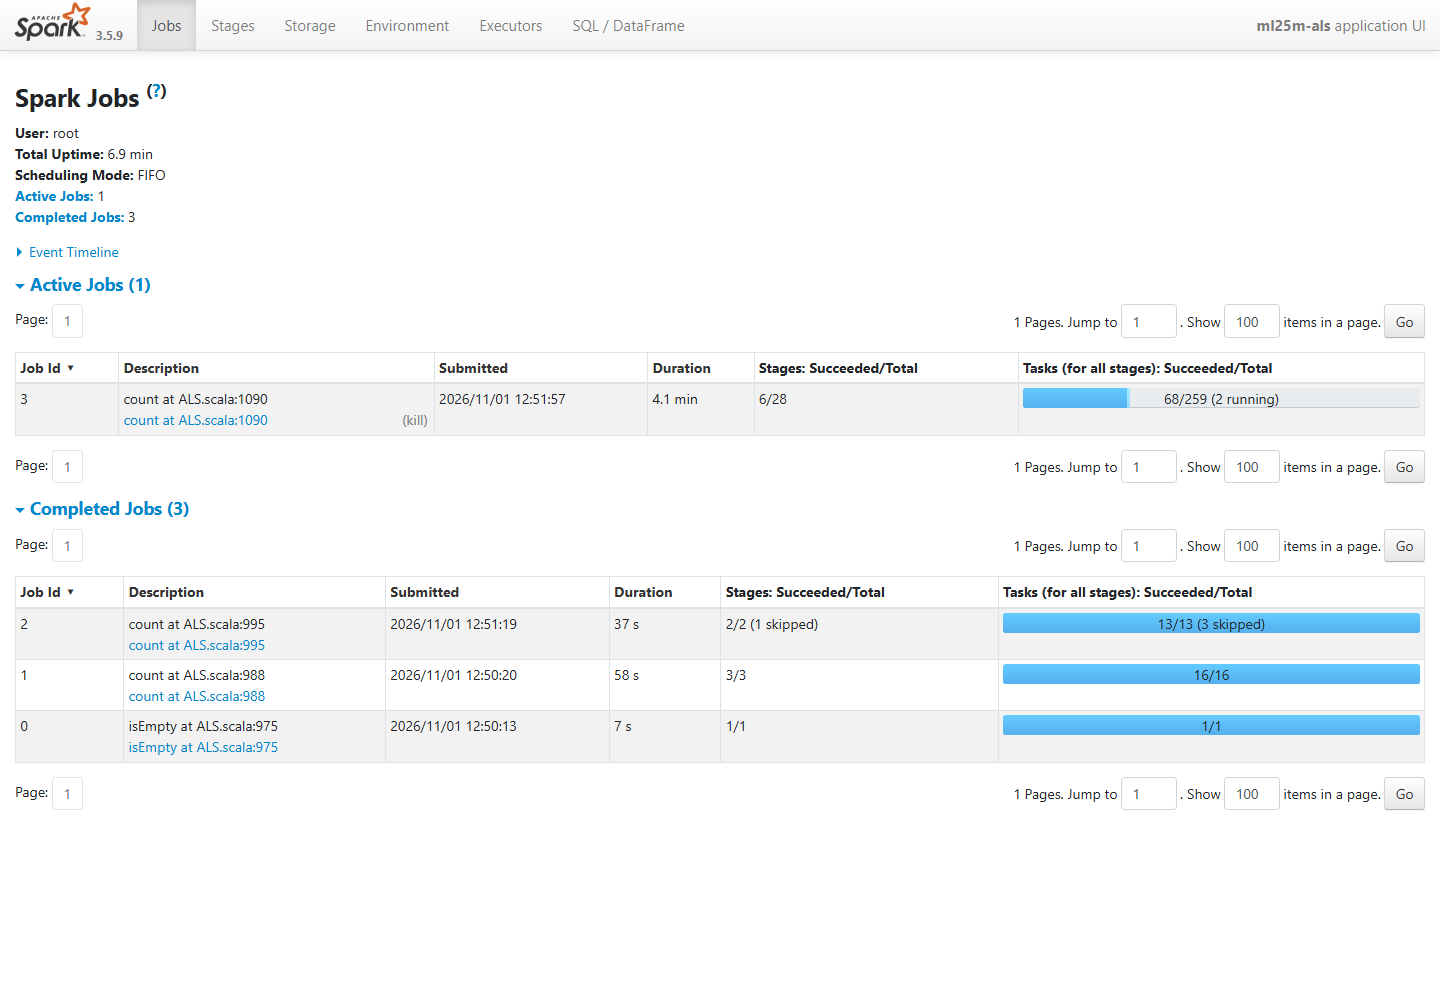
\includegraphics[width=\linewidth]{spark_jobs.png}\\[2pt]
    {\color{mute}\footnotesize ALS 训练中：259 个任务，活跃进度条在走}
    \column{0.49\textwidth}
    \centering
    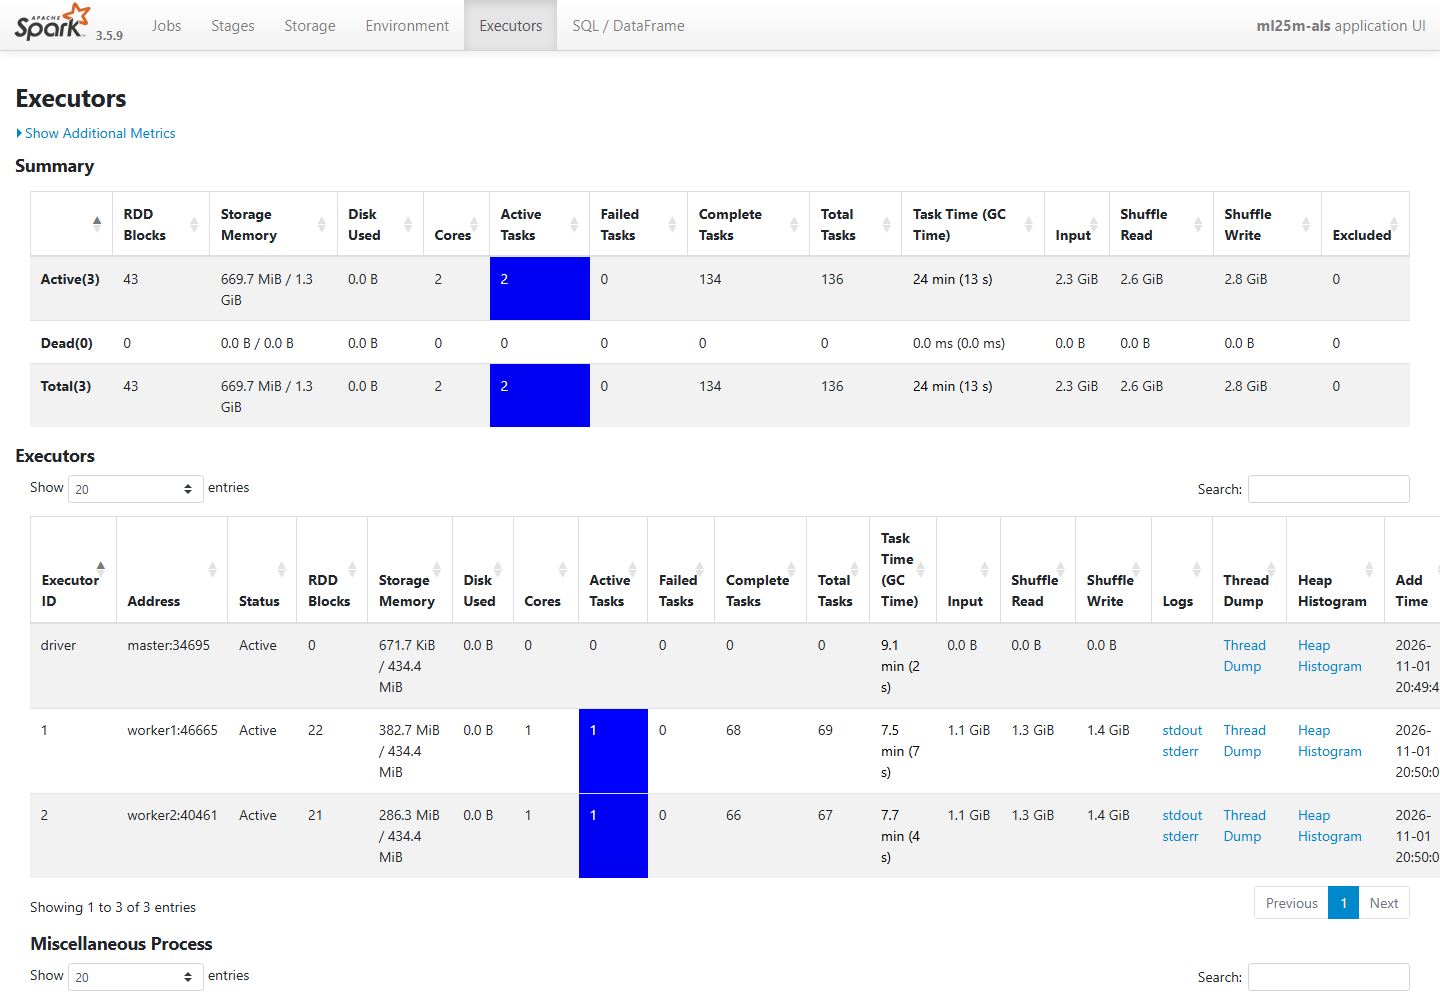
\includegraphics[width=\linewidth]{spark_executors.png}\\[2pt]
    {\color{mute}\footnotesize 两个执行器分工，shuffle 共 2.6GiB}
  \end{columns}
\end{frame}

% =====================================================
\divider{04}{项目总结}

\begin{frame}{值钱的部分，和换来的教训}
  \begin{columns}[T]
    \column{0.52\textwidth}
    \small
    \textbf{对着评分表交底}\\[2pt]
    \begin{itemize}
      \item 自建 Linux 环境：Docker 三节点，Hive 4 与 Spark 3.5 的兼容坑是亲手填的
      \item 复杂算法：SASRec、DeepFM、RQ 语义 ID、Trie 束搜索的生成式推荐
      \item 课外的活：faiss、ECharts、FastAPI、增量评测框架
      \item 每个零件都有消融数字，"为什么需要它"有数据支撑
    \end{itemize}
    \column{0.44\textwidth}
    \small
    \textbf{教训}\\[2pt]
    \begin{itemize}
      \item 显式评分学不会点击意图，隐式反馈建模才是对的
      \item 深度模型默认会过拟合，验证集挑检查点是标配
      \item 评测结果文件做成增量合并，重跑一个通道不会冲掉别的
      \item 版本不兼容时，保住"数据可查"比强求统一元数据更实际
    \end{itemize}
  \end{columns}
\end{frame}

\begin{frame}{没做完的，和下一步}
  \small
  \begin{itemize}
    \item GenRec 的数字：受制于 CPU，换 GPU 后加长序列、加训练轮数，再补物品内容特征
    \item 精排的天花板在特征：下一步上行为序列特征（DIN 式 target attention），而不是继续堆模型结构
    \item 现在是批训练 + 在线服务，缺一条实时链路：Flink 流式特征、定时刷新看板
    \item 只有离线消融，没有真实 A/B；可以先做基于重放的偏置校正评估
  \end{itemize}
  \vspace{10pt}
  \centering{\color{mute}\small 代码约 30 个源文件、5000+ 行，数据、模型、评测、服务四层齐全}
\end{frame}

% =====================================================
\divider{05}{成员分工}

\begin{frame}{成员分工}
  \small 本项目独立完成，以下全部由本人一人承担：
  \vspace{4pt}
  \centering\small
  \begin{tabular}{@{}p{0.78\textwidth}l@{}}
    \toprule
    模块 & 完成人 \\
    \midrule
    集群环境搭建（Hadoop / Hive / HBase / Spark on YARN） & 本人 \\
    数据管道（ETL、数仓分层、特征工程） & 本人 \\
    模型（ALS、ItemCF、SASRec、DeepFM、GBT、语义 ID、GenRec） & 本人 \\
    统一评测与消融实验框架 & 本人 \\
    在线服务与前端（FastAPI、ECharts） & 本人 \\
    实验报告与演示文稿 & 本人 \\
    \bottomrule
  \end{tabular}

  \vspace{10pt}\footnotesize\color{mute}
  开发过程用了 AI 编程助手辅助调试与代码生成；设计决策、实验结论和全部内容都经过本人验证。
\end{frame}

% =====================================================
\divider{06}{资源链接}

\begin{frame}{链接与复现}
  \small
  \textbf{在线}\\[2pt]
  \begin{itemize}
    \item 代码仓库：\alert{（GitHub/Gitee 链接，提交前填入）}
    \item 数据集：\mono{grouplens.org/datasets/movielens/25m/}
    \item 生成式推荐参考：TIGER（Google）、OneRec（快手）、\mono{github.com/LSH2003/MiniOneRec}
  \end{itemize}
  \vspace{8pt}
  \textbf{本地复现}\\[2pt]
  \begin{itemize}
    \item 数据与模型：\mono{spark/etl.py} $\to$ \mono{als.py} $\to$ \mono{samples.py} $\to$ \mono{gbt.py} $\to$ \mono{export.py}；\mono{models/} 与 \mono{sid/} 下是训练和评测脚本
    \item 起服务：\mono{python -m uvicorn serving.app:app --port 8000}，浏览器打开就是演示页
    \item 成绩单：\mono{experiments/summary.md}（总表）、\mono{experiments/screenshots/}（实况截图）
  \end{itemize}
\end{frame}

% ================= 结尾（暗页） =================
{\darkpage
\begin{frame}[plain]
  \vspace{10mm}
  {\color{darkfg}\fontsize{40}{44}\selectfont\bfseries 谢谢\textcolor{accent}{.}}\\[10pt]
  {\color{darkfg}\normalsize 系统现在还开着：\texttt{http://127.0.0.1:8000}\quad（参数 \mono{?uid=1\&q=科幻} 直达演示状态）}
  \vfill
  {\color{mute}\small （姓名 · 学号）\hfill 2026 年 11 月}
  \vspace{5mm}
\end{frame}}

\end{document}
